\documentclass{bio}
%\documentclass[oupdraft]{bio}
\usepackage[colorlinks=true, urlcolor=citecolor, linkcolor=citecolor, citecolor=citecolor]{hyperref}

% Add history information for the article if required
\history{}

\begin{document}

% Title of paper
\title{Methods that remove batch effects while retaining group differences may lead
to exaggerated confidence in downstream analyses
}

% List of authors, with corresponding author marked by asterisk
\author{VEGARD NYGAARD, EINAR ANDREAS R\O{}DLAND, EIVIND HOVIG$^\ast$\\[4pt]
% Author addresses
\textit{Department of Tumor Biology,
Institute for Cancer Research,
Oslo University Hospital HF - Radiumhospitalet,
Montebello,
0310 Oslo,
Norway}
\\[2pt]
% E-mail address for correspondence
{ehovig@radium.uio.no}}

% Running headers of paper:
\markboth%
% First field is the short list of authors
{V. Nygaard, E. A. R\o{}dland, E. Hovig}
% Second field is the short title of the paper
{Exagerated effects after batch correction}

\maketitle

% Add a footnote for the corresponding author if one has been
% identified in the author list
\footnotetext{To whom correspondence should be addressed.}

\begin{abstract}
{Removal of, or adjustment for, batch effects or centre differences is generally required when such effects are present in data. In particular, when preparing microarray gene expression data from multiple cohorts, array platforms, or batches for later analyses, batch effects can have confounding effects. Many methods and tools exist for this purpose. One method, ComBat which is part of the R package sva, is particularly popular due to its ability to remove batch differences even when batches are small and heterogeneous, while retaining the difference between study groups, e.g. treatments. Unfortunately, this recommended and frequently used approach to batch correction will systematically induce incorrect group differences in downstream analyses when groups are unevenly distributed between the batches. The scientific community seems to be largely unaware of this problem, which most likely has contributed to false discoveries being presented in the published literature.
}
\end{abstract}


%% NOTES TO SELF:
% Cite using:
%    \citet{...}  in text
%    \citealp{...}   within parantheses
%
% Temporary notifications and reminders:
\newcommand\NB[1]{{\color{red}#1}}
\newcommand\NOTE[1]{{\color{red}[#1]}}
\newcommand\CITE[1]{{\color{magenta}[#1]}}

\section{Introduction}\label{intro}

Extraneous variables, if left unaccounted for, have the potential to lead an investigator into drawing wrong conclusions. In molecular biology, extraneous variables are often called "batch effects", probably due to the fact that reagents and other equipment, for instance microarray chips, are made in batches, and this is frequently observed as an effect in the measurements. See 20676067 for more examples. 

For a typical experiment comparing group differences, the presence of batch effects will decrease the statistical power. If the batch/group design is unbalanced - i.e the proportion of one groups samples belonging to each batch is not equal for all groups - batch may act as a confounder and lead to false positive results as well (20838408).

The standard way to handle an extraneous variable is to include it in the statistical model employed in the inquiry. However, many analytic tools for high throughput data does not cater for this option, and when available it could still be outside the competence of the investigator. Therefore, an alternative two step procedure has emerged, first the batch effects are estimated and removed, creating a "batch effect free" data set. In the next step, the statistical analysis is performed on the adjusted data as there never were batch effects in the first place. This appealing compartmentalization is also convenient for practical purposes, for example when data-processing and statistical analyses are performed by different personnel.

The first step can be achieved by subtracting the mean of the measurements in one batch from all measurements in that batch, i.e mean adjustment or one-way ANOVA adjustment as implemented in the method pamr.batchadjust from the pamr package in R. When the batch/group design is balanced, mean-adjustment will take out some, but not necessarily all, variance attributed to batch and leave the between group variance, thus increasing the statistical power. However, when batch is a confounder, some of the variance removed will be group variance and statistical power will be lost. In addition if there are many groups, some effect will be transferred between groups that share batches, leading to false positive results. \NOTE{Dette problemet er ikke beskrevet i de andre artiklene eller i einars mail, men saa vidt jeg skjoenner saa kan dette skje.}

To mitigate the above problems, group differences can, simplified explained, be estimated based on the balanced part of the data and applied to all samples in the adjusted data set. If all the samples, and not only the balanced ones, are used as sample size in later a group comparison, the confidence will be overestimated.

The ComBat method described in 16632515 and also included in the sva package (22257669) implements the above described procedure in an attempt to retain group differences when adjusting for batch effects. Based on actual use of ComBat by the authors and others, we suspect the adjusted data predominantly is treated as "batch effect free" in the subsequent analysis. And as a consequence, confidence is overestimated and false results are reported.

\NB{Kort oppsummere behovet for batch-korrigering: generelt og i microarraydata.}

\NB{Kort beskrive metoder som gjoer dette (batch-sentrering, ANOVA, ComBat).}

\NB{Forklare tilsiktet effekt disse paa batch+gruppe-forskjeller (balansert versus ikke-balansert).}

\NB{Forklare kort hva faktisk effekt er: ANOVA gir redusert gruppe-forskjeller, mens for ComBat overestimeres den statistiske styrken/sikkerheten av forskjellen.}


\section{Methods for batch effect correction}

\subsection{Model for data with batch effects}

We will base out discussion of data with batch effects on a simple model:
\begin{equation}
Y_{ijr}=\alpha+\beta_j+\gamma_i+\epsilon_{ijr}
\end{equation}
where $i=1,\ldots,m$ are the different batches, $j=1,\ldots,M$ are different study groups that we wish to compare, and $r=1,\ldots,n_{ij}$ are the different samples within batch $i$ and group $j$.

When combining data from more diverse data sources, e.g. microarray data from different platforms, a more general model is required. One such model, used by \CITE{ComBat}, is
\begin{equation}
Y_{ijgr}=\alpha_g+X_r\beta_{g}+\gamma_{ig}+\delta_{ig}\epsilon_{ijgr}
\end{equation}
where $g=1,\ldots,G$ are different measurements, e.g. genes, performed for each sample, and $X$ is the design matrix which in our case will indicate the study group. This permits independent rescaling of data from different batches. In addition, \CITE{ComBat} uses an empirical Bayes approach to estimate $\gamma_{ig}$ and $\delta_{ig}$ to stabilise estimates, which is critical for use with small batches.

For simplicity, we consider the case with a single gene and constant scale, i.e. $\delta_{ig}=1$. We will discuss the effect of empirical Bayes estimation of $\gamma_{ig}$ later, but out main argument is more easily made in the simpler context.

\subsection{Standard batch correction methods}

The main ambition of batch effect adjustments is to be able to remove batch differences in such a way that downstream analyses of the adjusted data may be done without further batch adjustments.

The most common method for removing batch effects is to zero-centre each batch:
\begin{equation}
\Delta\widetilde Y_{ijr}=Y_{ijr}-\overline{Y}_{i}
\quad\text{where}\quad
\bar Y_i=\frac{\sum_{j=1}^M\sum_{r=1}^{n_{ij}} Y_{ijr}}{\sum_{j=1}^M n_{ij}}.
\end{equation}
An alternative is to centre each batch to the common average by adding the average value $\bar Y$ across the entire data set: i.e. $\widetilde Y_{ijr}=\Delta\widetilde Y_{ijr}+\bar Y$. When comparing groups, the common value $\bar Y$ has no effect, and so this is equilvalent to zero-centring each batch. However, if the different groups are unevenly represented in the different batches, the batch average $\overline{Y}_i$ will tend to capture group differences as well as batch effects. Thus, batch centering may reduce group differences, and thus reduce the power of downstream analyses.

Removing batch effects while retaining group differences can be done through an ANOVA analysis in which the group effects, $\beta_j$, and the batch effects, $\gamma_i$, are estimated simultaneously. Batch adjusted values may then be obtained by subtracting the estimated batch effects, $\hat\beta_j$:
\begin{equation}
\widetilde Y_{ijr}=Y_{ijr}-\hat\beta_j=\alpha+(\beta_j-\hat\beta_j)+\gamma_i+\epsilon_{ijr}.
\end{equation}
This will yield batch adjusted values where any systematic bias induced by the batch differences has been removed, while the group differences are retained.

Unfortunately, the estimation error $\hat\beta_j-\beta_j$ affects all values within the same batch in the same manner, inducing a dependency between the values. If the study groups are evenly represented in all batches, this will not influence estimated group differences as all groups are equally affected. However, if groups are unevenly represented, this induced dependency can have severe impact on downstream analyses.


\section{Results}

\subsection{A simple sanity check}

The undesired consequences of preserving group effects when correcting for batch effect is readily illustrated with a sanity check using random numbers . The documentation accompanying the sva library has a runnable example demonstrating how to adjust a data set with ComBat followed by a F-test. Swapping the real data with random numbers from a normal distribution (mean=0, sd=1), but otherwise following the instructions, will generate the p-value distribution shown in Figure 1. The skewed distribution is a indication that this approach may have a unintentional adverse effect. \NOTE{Jeg har ikke beskrevet permutatsjon checken fordi jeg er usikker paa om vi skal bruke den.}

%% FIGURE 1: Original position

\NB{Formler og ord:
Forklare hva som gaar galt med formler og ord. Overlater til Einar aa skrive dette.}

\subsection{Examples of undesired consequences}

As the amount of false positive results when trying to retain group differences depends on the batch/group balance, we will show two examples with varying degree of unbalancedness. 

1) In the first experiment(24421904), cells were treated with glatiramer acetate (a medicine for multiple sclerosis) or a generic and mRNA was measured using microarrays alongside control samples. A batch effect correlating to the chip (Illumina WG-6\_V2, six samples per chip) was observed and adjusted for with ComBat, whereafter the data was tested for differetially expressed genes, yielding a list of 1000 genes (Table S5 24421904). Unfortunately the batch/treatment design was unbalanced with several batches having only one of the main treatments of interest. When we re-analyzed their data without using ComBat, but instead blocked for batch effect in limma, only 9 genes were found (FDR<0.05). Additional sanity checks with random numbers or perumted labels were also carried out and the distribution of p-values for differents settings are shown in Fig. 2.  Our conclusion is that most of the genes reported as differtially expresssed in (24421904) are false positives. This example is a sort of "worst case" scenario for applying ComBat, since it both has a very unbalanced batch/group design and a a priori assumpotion of no difference. The R-code for our analysis and a more extensive report can be downloaded from github (\href{https://github.com/vegardny/combat_tests.git}).

%![fig. 2](../reanalysis/Fadi_Towfic_generic_medicine/figure/pvaluestowfic.svg)
%**Figure 2**.
%P-value distribution for the main comparison in (data set 2 24421904) glatiramer acetate vs. generic.  
%- a) Real data adjusted by ComBat as described in the article followed by a significance test in limma. 
%- b) Real data not adjusted by ComBat, tested for significance in limma using batch as a blocking factor. 
%- c) Real data is substituted with random numbers from a normal distribution (mean=0, sd=1), but the batch/group design is retained, followed by batch adjustment in ComBat and a significance test in limma.
%- d) 10 runs of real data with the glatiramer acetate("DP") and generic("N") labels permuted within batches, followed by ComBat adjustment and significance test in limma.  
%_jeg tok med begge sanitycheckene her. Er d) slik einar foreslo?. Merk jeg har ikke permutert alle labeler, bare de mellom DP og N. Det er en del andre._

2) The second example is taken from the supporting information for the original ComBat article (16632515) where it is denoted "data set 2". Cells inhibited for the expression of the TAL1 gene were compared to controls on a microarray platform. The experiment was conducted on three different time points (used as batches) with a total of 30 samples and a fairly balanced batch/treatment set up (6-2, 3-4 and 9-6). ComBat was applied followed by a t-test in order to identify differentially expressed genes. First, we reproduced their analysis including the adjustment by ComBat, but using limma instead of the t-test, resulting in 1003 probes (q<0.05).  Then, we analysed their data without batch adjustment in ComBat, but blocking for batch in limma, resulting in 377 probes (q<0.05). In addition the two sanity checks outline above were performed. In contrast to the above results obtained for(24421904), the P-value distributions for the alternative analyses (Fig.3 a,b) does not indicate a huge difference. Nevertheless, we belive that  P-values are deflated for the ComBat adjusted analysis. The R-code for our analysis and a more extensive report can be downloaded from github (\href{https://github.com/vegardny/combat_tests.git}).

%![fig. 3](../reanalysis/ComBat_original/figure/pvaluesjohnson.svg)  
%**Figure 3**.
%P-value distribution for the main comparison in (data set 2 16632515) for  
%- a) Real data adjusted by ComBat as described in the article followed by a significance test in limma. 
%- b) Real data not adjusted by ComBat, tested for significance in limma using batch as a blocking factor. 
%- c) Real data is substituted with random numbers from a normal distribution (mean=0, sd=1), but the batch/group design is retained, followed by batch adjustment in ComBat and a significance test in limma.
%- d) 10 runs of real data with the group labels permuted within batches, followed by ComBat adjustment and significance test in limma.   
%_problemet med permutatsjons sanitychechen slik jeg har utfoert og plottet den her er at den neppe kan sies aa feile. Dessuten kan de 3 foerst plottene bli plottet i ett som vist under i en alternativ version jeg synes er finere, men dette gaar ikke for permutasjonstesten tror jeg_

%![fig. 4](../reanalysis/ComBat_original/figure/pvaluesjohnson2.svg)   
%_Alternativ illustrasjon av de tre p-value distribusjonene_


3) \NOTE{Her kan vi fylle paa med flere eksempler etter samme mal hvis det trengs. Feks en fersk artikkel fra Nature Genetic([24584070](http://www.nature.com/ng/journal/vaop/ncurrent/full/ng.2916.html)). Der har de kombinert sekvenseringsdata  (deres data) fra 9 lymfom pasienter med et (eksternt) microarray data set som har 6 lymfom proever og 5 kontroller, dvs kontroll gruppen er helt fravaerende hos dem. Dvs veldig ubalansert (9/0, 6/5), MEN skille mellom phenotypene er saa stor at de sikkert hadde funnet omtrent de samme genene signifikante med aa bare bruke de balanserte dataene (men det var jo ikke deres.) Dette er ikke en viktig del av paperet, men det er veldig feil selvom konsekvensense ikke blir store. Dog gir det et falskt inntrykk av at dataene deres ligner tidligere data, se heatmap i suppl.. Dessuten lager de GO analyser av dette som egentlig er 7 aar gamle andres data og ikke deres}


\section{Discussion}

\subsection{Increased emphasis on preserving group difference}

In the original ComBat article(2007) it is clear that the primary motivation behind ComBat was to employ an Emprical Bayes method for batch-effect removal. The feature of retaining group differences for unbalanced designs is optional and seems to be subordinate, only exemplified in the supplementary information. However, over the years this feature became more important judging from advice given by the author to users
(
[1](\href{https://groups.google.com/d/msg/combat-user-forum/eSVSKwGtuyE/ZIWV2juYmmAJ})
,[2](\href{https://groups.google.com/d/msg/combat-user-forum/Vkb9p7wekd4/h5Etie7FTVQJ})
,[3](\href{https://groups.google.com/d/msg/combat-user-forum/fpBTcgDjiR8/uo4QIZL4sZgJ})
,[4](\href{https://groups.google.com/d/msg/combat-user-forum/26FZlgU2LFQ/W6U_Lhh_64EJ})
). \NOTE{Aa linke direkte er kanskje litt ufint, alternativt kan det linkes til forumet uten konkrete innlegg.}  
And when ComBat was incorporated in the sva package ( [22257669](\href{http://bioinformatics.oxfordjournals.org/cgi/pmidlookup?view=long&pmid=22257669}), 2012), inclusion of group labels was made almost mandatory (an undocumented option of passing a NULL value exists). Thus, this problematic use has likely been common.


\subsection{Motivation for this warning}

Our knowledge of ComBat came through a typical use case when trying to salvage unbalanced data which had batch effects. Upon realizing that the confidence on our group differences were exaggerated, the literature was searched for a better understanding of correct use and potential overseen limitations of ComBat. But the authors of ComBat and the sva package recommended our usage (16632515, 22257669). In addition, other works looking into the problem of batch effects were mostly recommending ComBat without much concern (22682473, 22133085). A brief inquiry into  some of the articles citing ComBat (574 Google Scholar) revealed few problems, and their method descriptions regarding ComBat were mostly sparse, limited to one or two sentences (24391845, 18414638, 21731603,23630272, 24584070). A further indication of their carefree use of this potentially devastating procedure was the frequent neglect to state the program parameters, i.e batch labels (18414638, 21731603) or group labels (24391845, 18414638, 21731603, 23630272, 23482648, 24584070). Often no effort was done in order to substantiate the existence of batch effects in their data, except for stating the presence of batches (24391845?, 18414638, 21731603, 23630272). In one instance ComBat was even applied on data were effects due to batch were investigated, but not found \NOTE{husker ikke ref}. The incorporation of the method into analysis pipelines (16642009,TCGA) and other packages (23452776, 21937664) could make its usage even more trivial and parameters setting harder to perceive.
Taken together we fear that many published results from data adjusted by ComBat are completely or partially false. And knowing that scientists don't give up where one analysis fails, a method that almost ensures a result given a sufficiently unbalanced design will continue to be used.


\subsection{Practical advice}

We have shown that adjusting for batch effects while preserve the group difference may lead to varying degree of false results. Knowing this, to what degree can an investigator trust a result from a work applying such a method? Essentially, when the batch/group configuration is balanced, or group difference is ignored  (i.e. no group labels not given as parameters to ComBat), problems related to preserving group differences will not occur. For other cases, a re-analysis without using this approach is the most rigorous path. However, this thoroughness is not feasible if the downstream  analysis can not adjust for batch effects by it self. To reach a reliable result, batch effects need to be handled in some way or another. To make matters worse, a re-analysis relies on the availability of the raw data and a description of processing and analysis steps taken in the original work. Even when this is available, the necessary bioinformatic skills and work hours could still be in short supply. For such situations, a superficial assessment can be performed, taking special note of batches were groups of interest are near missing and how likely a group difference is. In essence asking if the balanced parts (effective sample size?) of the data has enough power to detect the presumed effects and if this is the case (16632515, 24584070), treat the results more like an ordered list with the most likely true positives on top while de-emphasizing the somewhat deflated p-values . In contrast, if biological knowledge suggest that a group effect is unlikely  (24391845, 18414638?, 21731603, 23630272), an intermediate lack of batch/group balance  could lead to a mostly false result.

\subsection{Reproducible research}
\NOTE{vi boer klare aa tilfredstille kravene i http://biostatistics.oxfordjournals.org/content/10/3/405.full}


\section{Supplementary Material}
\label{supp}

Supplementary material is available online at
\href{http://biostatistics.oxfordjournals.org}%
{http://biostatistics.oxfordjournals.org}.


\section*{Acknowledgments}

[...Acknowledgements...]
{\it Conflict of Interest}: None declared.


\bibliographystyle{biorefs}
\bibliography{refs}


%\begin{figure}[!p]
%\centering\includegraphics{fig1.eps}
%\caption{...}
%\label{Fig1}
%\end{figure}

\begin{figure}[!p]
\centering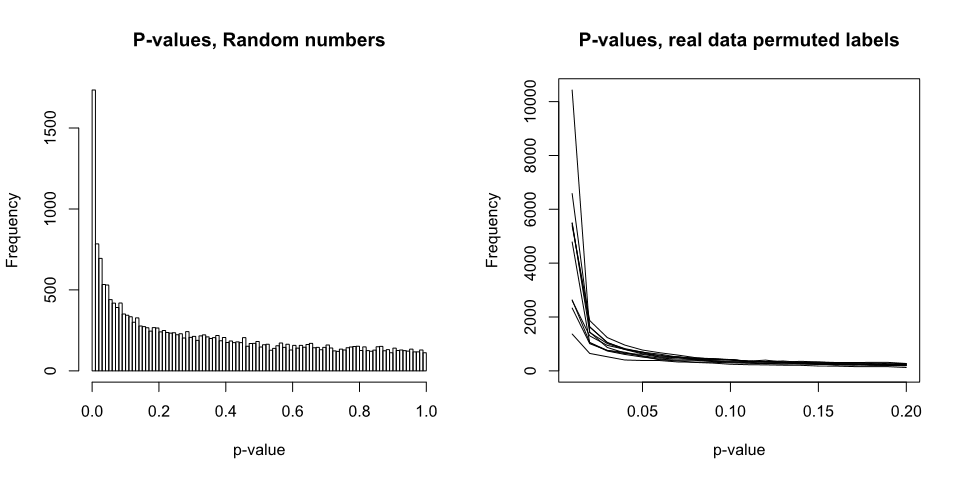
\includegraphics[width=15cm]{Fig/pvaluesleeksva.png}
\caption{
Two sanity checks were the recommended use of ComBat fails. Adapted from the user guide in the sva package. 
a) Real data is substituted with random numbers from a normal distribution (mean=0, sd=1), but the batch/group design is retained, followed by batch adjustment in ComBat and a F-test.
b) 10 runs of real data with the "cancer" labels permuted within batches, followed by ComBat adjustment and a F-test. All permutations produces a skewed p-value distribution.
}
\label{Fig1}
\end{figure}

%![fig. 1](../reanalysis/leek_sva/figure/pvaluesleeksva.svg)  
%**Figure 1**  


%\begin{table}[!p]
%\tblcaption{... \protect\citet{...} ... \label{Table1}}
%{\tabcolsep=4.25pt
%\begin{tabular}{@{}cccccccccc@{}}
%\tblhead{Dis & Chr & Marker & MLE-OR & MLE & MLE & EB-HM-OR & EB-HM & EB-HM & ES \\
%&&& (SE) & \textit{P}-value & rank & (SE) & \textit{P}-value & rank & rank}
%CAD & 2 & rs2943634 & 1.22(0.04) & $1.23 \times 10^{-5}$ & 32 & 1.02(0.01) & 0.19 & 28 & 37 \lastline
%\end{tabular}}
%\end{table}

\end{document}

